\chapter{Infraroodspectroscopie}\label{ch:g11:infrared}

Op een plank in het laboratorium staat een fles kleurloze vloeistof
waarvan het etiket is afgescheurd. Het kan een \omterm{def:g11:functional-groups:alcohol}{alcohol} zijn, een \omterm{def:g11:functional-groups:carbonyl}{keton}
of een zuur: drie families die er in een fles precies hetzelfde uitzien.
Een druppel op het kristal van een infraroodspectrometer, twee minuten
wachten, en er verschijnt een grafiek op het scherm die de vraag
beantwoordt. De bindingen van een \omterm{def:g7:atoms-and-molecules:molecule}{molecuul} trillen, en elke soort binding
neemt infrarood licht van haar eigen frequenties op: een
\omterm{def:g11:infrared:spectrum}{infraroodspectrum} is een lijst van de aanwezige bindingen.

\begin{recall}
\omterm{def:g11:functional-groups:functional-group}{Karakteristieke groepen} en families (\cref{ch:g11:functional-groups}).
Een \omterm{def:g11:absorbance:spectrum}{absorptiespectrum} laat zien hoeveel licht een stof bij elke
golflengte opneemt (\cref{ch:g11:absorbance}). \omterm{def:g11:polarity-and-cohesion:hydrogen-bond}{Waterstofbruggen} verbinden
\ce{O-H}-groepen met naburige \omterm{def:g7:atoms-and-molecules:molecule}{moleculen}
(\cref{ch:g11:polarity-and-cohesion}).
\end{recall}

\section{Bindingen trillen}

Een \omterm{def:g10:lewis-and-shape:covalent-bond}{covalente binding} is niet star: de twee \omterm{def:g7:atoms-and-molecules:atom}{atomen} trillen, bewegen
vele miljoenen miljoenen keren per seconde naar elkaar toe en van elkaar
af, zoals twee balletjes verbonden door een veer. Een stijvere veer (een
\omterm{def:g10:lewis-and-shape:multiple-bond}{dubbele binding} in plaats van een enkele) of lichtere balletjes (een
waterstofatoom in plaats van een koolstofatoom) trillen sneller. Een
binding kan infrarood licht opnemen waarvan de frequentie overeenkomt
met haar eigen trilling: infrarood licht, onzichtbaar voor het oog, heeft
golflengten van een paar micrometer tot een paar tientallen micrometer.

\begin{omfigure}
\begin{tikzpicture}[font=\small]
  \node[aC] (c) at (0,0) {};
  \node[aO] (o) at (2.2,0) {};
  \draw[decorate, decoration={coil, aspect=0.4, segment length=4pt,
    amplitude=4pt}, thick, black!60] (c.east) -- (o.west);
  \draw[<->, omProp, thick] (-0.9,0) -- (-0.45,0);
  \draw[<->, omProp, thick] (2.65,0) -- (3.1,0);
  \node[anchor=north] at (1.1,-0.5) {een binding die uitrekt en inkrimpt};
  \node[aO] (o1) at (5.3,0) {};
  \node[aH] (h1) at (6.7,0) {};
  \draw[decorate, decoration={coil, aspect=0.4, segment length=3pt,
    amplitude=3pt}, thick, black!60] (o1.east) -- (h1.west);
  \draw[<->, omProp, thick] (7.0,0) -- (7.7,0);
  \node[anchor=north, align=center] at (6.2,-0.5) {een licht waterstofatoom:\\ snellere trilling};
\end{tikzpicture}

{\small Een binding voorgesteld als een veer tussen twee balletjes. De
trilling heeft een frequentie die bepaald wordt door de stijfheid van de
binding en de massa's van de \omterm{def:g7:atoms-and-molecules:atom}{atomen}; infrarood licht met die frequentie
wordt opgenomen.}
\end{omfigure}

\begin{definition}[Golfgetal]\label{def:g11:infrared:wavenumber}
Het \emph{golfgetal}\index{golfgetal} $\sigma$ van licht is het omgekeerde
van de golflengte, $\sigma = 1/\lambda$. In de infraroodspectroscopie
wordt het uitgedrukt in \si{cm^{-1}}: het aantal golflengten in één
centimeter. Een groter golfgetal betekent een kortere golflengte en een
snellere trilling.
\end{definition}

\begin{example}[Van een golfgetal naar een golflengte]\label{ex:g11:infrared:convert}
Een band bij $\sigma = \qty{2000}{cm^{-1}}$ hoort bij
$\lambda = 1/2000 = \qty{5.0e-4}{cm} = \qty{5.0}{\micro m}$.
\omterm{def:g11:infrared:spectrum}{Infraroodspectra} lopen meestal van \qty{4000}{cm^{-1}}
(\qty{2.5}{\micro m}) tot \qty{500}{cm^{-1}} (\qty{20}{\micro m}).
\end{example}

\section{Een infraroodspectrum lezen}

\begin{definition}[Infraroodspectrum, transmissie]\label{def:g11:infrared:spectrum}
De \emph{transmissie}\index{transmissie} $T$ van een monster bij een
gegeven \omterm{def:g11:infrared:wavenumber}{golfgetal} is het percentage van het infrarode licht dat erdoorheen
gaat: \qty{100}{\percent} als er niets wordt opgenomen. Het
\emph{infraroodspectrum}\index{infraroodspectrum} van een verbinding is
de grafiek van $T$ uitgezet tegen het \omterm{def:g11:infrared:wavenumber}{golfgetal}, volgens afspraak
getekend met de \omterm{def:g11:infrared:wavenumber}{golfgetallen} afnemend van links naar rechts.
\end{definition}

\begin{definition}[Absorptieband, vingerafdrukgebied]\label{def:g11:infrared:band}
Een \emph{absorptieband}\index{absorptieband} is een dip in de
\omterm{def:g11:infrared:spectrum}{transmissie}: het licht met die \omterm{def:g11:infrared:wavenumber}{golfgetallen} wordt door een binding
opgenomen. De plaats ervan zegt welke binding het is, de breedte en de
diepte vullen het beeld aan. Onder ongeveer \qty{1500}{cm^{-1}} staat het
spectrum vol banden die van het hele \omterm{def:g7:atoms-and-molecules:molecule}{molecuul} afhangen: dit
\emph{vingerafdrukgebied}\index{vingerafdrukgebied} identificeert een
verbinding door vergelijking met een bekend spectrum, maar is moeilijk
binding voor binding te lezen.
\end{definition}

\begin{inthelab}[Een spectrum opnemen]
De meeste spectrometers op school en aan de universiteit gebruiken nu een
klein diamantkristal: een druppel vloeistof, of een paar korrels vaste
stof die met een klem worden aangedrukt, wordt op het kristal gelegd, en
de infraroodbundel die langs het oppervlak strijkt, onderzoekt het
monster. Eerst wordt het schone kristal opgenomen (de
``achtergrond''), die de rol van de blanco speelt. Tussen twee monsters
wordt het kristal schoongemaakt met een tissue en een beetje
\omterm{def:g6:solutions-and-solubility:solute}{oplosmiddel}.
\end{inthelab}

\section{Kenmerkende banden}

\begin{proposition}[Elke soort binding heeft haar band]\label{prop:g11:infrared:bands}
% ledger: ir:OH-free, ir:OH-bonded, ir:OH-acid, ir:NH, ir:CH, ir:CO-aldehyde, ir:CO-ketone, ir:CO-ester, ir:CO-acid, ir:CC-double, ir:CO-single
Elke soort binding absorbeert in een kenmerkend gebied van \omterm{def:g11:infrared:wavenumber}{golfgetallen},
dat van \omterm{def:g7:atoms-and-molecules:molecule}{molecuul} tot \omterm{def:g7:atoms-and-molecules:molecule}{molecuul} bijna hetzelfde is:
\begin{center}
\small
\begin{tabular}{lll}
\hline
binding & \omterm{def:g11:infrared:wavenumber}{golfgetal} (\si{cm^{-1}}) & uiterlijk \\
\hline
\ce{O-H}, zonder \omterm{def:g11:polarity-and-cohesion:hydrogen-bond}{waterstofbrug} (gas, verdund) & bij 3600 & smal \\
\ce{O-H}, met \omterm{def:g11:polarity-and-cohesion:hydrogen-bond}{waterstofbrug} (vloeibare \omterm{def:g11:functional-groups:alcohol}{alcohol}) & 3300--3400 & breed, sterk \\
\ce{O-H} van een \omterm{def:g11:functional-groups:carboxylic-acid}{carbonzuur} & 2500--3300 & heel breed \\
\ce{N-H} van een \omterm{def:g11:functional-groups:amine}{amine} & 3300--3500 & matig (twee banden bij \ce{-NH2}) \\
\ce{C-H} van een keten & 2850--2960 & sterk \\
\ce{C=O} van een \omterm{def:g11:functional-groups:carboxylic-acid}{ester} & bij 1735 & heel sterk, smal \\
\ce{C=O} van een \omterm{def:g11:functional-groups:carbonyl}{aldehyde} & bij 1730 & heel sterk, smal \\
\ce{C=O} van een \omterm{def:g11:functional-groups:carbonyl}{keton} & bij 1715 & heel sterk, smal \\
\ce{C=O} van een \omterm{def:g11:functional-groups:carboxylic-acid}{carbonzuur} & bij 1710 & heel sterk, breder \\
\ce{C=C} & bij 1650 & matig \\
\ce{C-O} van een \omterm{def:g11:functional-groups:alcohol}{alcohol} & bij 1050 & sterk \\
\hline
\end{tabular}
\end{center}
\end{proposition}

\begin{proof}
Deze gebieden zijn gemeten aan veel verbindingen (ledger). Ze zijn per
binding gegroepeerd omdat de trilling van een binding vooral afhangt van
de binding zelf en haar twee \omterm{def:g7:atoms-and-molecules:atom}{atomen}, en weinig van de rest van het
\omterm{def:g7:atoms-and-molecules:molecule}{molecuul}.
\end{proof}

\begin{omfigure}
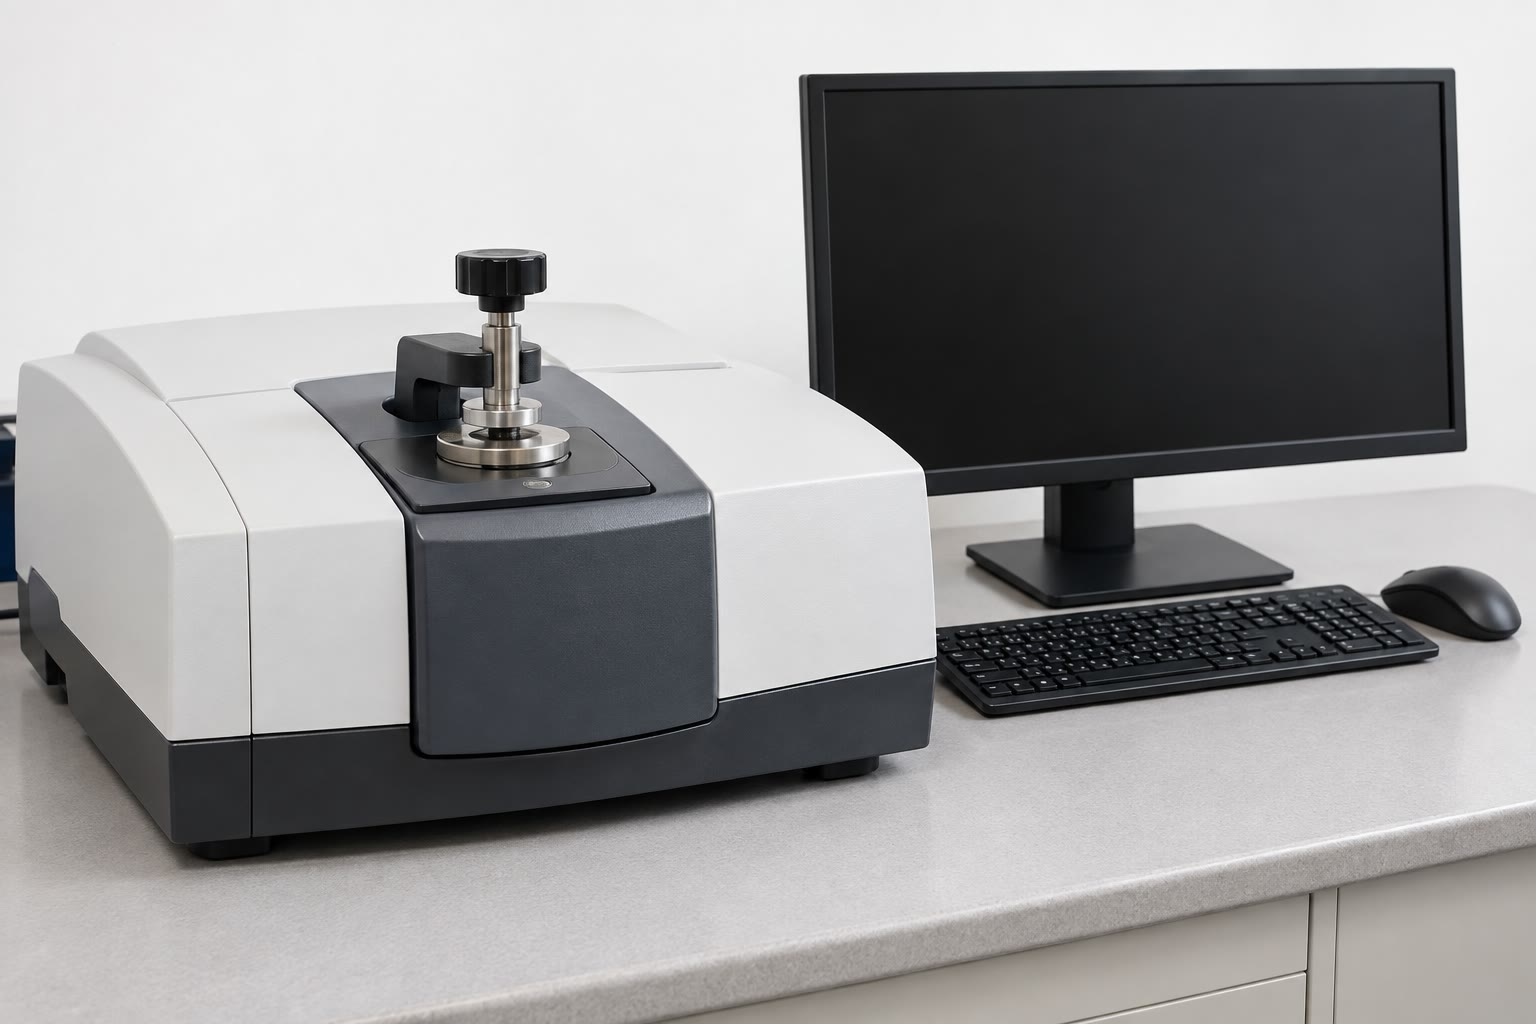
\includegraphics[width=0.48\linewidth]{images/book1/ai/g11-ftir.jpg}

{\small Een infraroodspectrometer voor op de labtafel, met zijn kristal en
klem.}
\end{omfigure}

\begin{omfigure}
\begin{tikzpicture}[font=\small, x=0.0036cm, y=0.5cm]
  % wavenumber axis reversed: x = 4000 - sigma
  \fill[black!8] (2500,0.2) rectangle (3500,7.6);
  \node[font=\footnotesize, align=center, black!60] at (3000,6.8) {vingerafdruk-\\ gebied};
  \draw[->] (0,0) -- (3600,0) node[right] {$\sigma$};
  \foreach \s in {4000,3500,3000,2500,2000,1500,1000,500}
    \draw ({4000-\s},0) -- ({4000-\s},-0.15) node[below, font=\footnotesize] {\s};
  \node[below=12pt] at (1800,-0.3) {golfgetal (\si{cm^{-1}})};
  \foreach \a/\b/\y/\c/\l in {
      3600/3600/7/omDef/{\ce{O-H} vrij},
      3300/3400/6/omDef/{\ce{O-H} gebonden},
      2500/3300/5/omThm/{\ce{O-H} zuur},
      3300/3500/4/omMeth/{\ce{N-H}},
      2850/2960/3/black!60/{\ce{C-H}},
      1700/1740/2/omProp/{\ce{C=O}},
      1050/1050/1/black!45/{\ce{C-O}}} {
    \fill[\c, rounded corners=1pt] ({4000-\b-12},{\y-0.25}) rectangle ({4000-\a+12},{\y+0.25});
    \node[anchor=west, font=\footnotesize] at ({4000-\a+40},\y) {\l};
  }
\end{tikzpicture}

{\small Waar de belangrijkste bindingen absorberen. De \ce{O-H}- en
\ce{N-H}-banden liggen links, de \ce{C=O}-band, meestal de sterkste, bij
\qty{1700}{cm^{-1}}; onder \qty{1500}{cm^{-1}} ligt het
\omterm{def:g11:infrared:band}{vingerafdrukgebied}.}
\end{omfigure}

\begin{proposition}[Waterstofbruggen verbreden de O--H-band]\label{prop:g11:infrared:hbond}
% ledger: ir:OH-free, ir:OH-bonded, ir:ethanol-OH
Als \ce{O-H}-groepen door \omterm{def:g11:polarity-and-cohesion:hydrogen-bond}{waterstofbruggen} verbonden zijn, zoals in een
vloeibare \omterm{def:g11:functional-groups:alcohol}{alcohol}, is hun band breed en ligt ze bij lagere \omterm{def:g11:infrared:wavenumber}{golfgetallen}
(ongeveer 3300--\qty{3400}{cm^{-1}}); zonder \omterm{def:g11:polarity-and-cohesion:hydrogen-bond}{waterstofbruggen}, zoals in het
gas, is ze smal en ligt ze bij \qty{3600}{cm^{-1}}.
\end{proposition}

\begin{proof}
Aangenomen: een \omterm{def:g11:polarity-and-cohesion:hydrogen-bond}{waterstofbrug} trekt aan het waterstofatoom en maakt de
\ce{O-H}-binding losser, zodat die langzamer trilt; en omdat elk \omterm{def:g7:atoms-and-molecules:molecule}{molecuul}
een beetje anders gebonden is, spreidt de band zich over een gebied.
\end{proof}

\section{Karakteristieke groepen herkennen}


\begin{method}[Een infraroodspectrum lezen]\label{met:g11:infrared:reading}
\begin{enumerate}
  \item Kijk eerst boven \qty{1500}{cm^{-1}}; bewaar het
        \omterm{def:g11:infrared:band}{vingerafdrukgebied} voor een vergelijking met bekende spectra.
  \item Bij \qty{1700}{cm^{-1}}: een heel sterke band betekent een
        \ce{C=O}-groep (\omterm{def:g11:functional-groups:carbonyl}{aldehyde}, \omterm{def:g11:functional-groups:carbonyl}{keton}, zuur, \omterm{def:g11:functional-groups:carboxylic-acid}{ester}, \omterm{def:g11:functional-groups:amine}{amide}).
  \item Tussen 2500 en \qty{3700}{cm^{-1}}: een brede band bij
        \qty{3350}{cm^{-1}} betekent een alcohol-\ce{O-H}; een heel brede
        band van 2500 tot \qty{3300}{cm^{-1}} samen met een \ce{C=O}
        betekent een \omterm{def:g11:functional-groups:carboxylic-acid}{carbonzuur}; middelmatige banden bij
        3300--\qty{3500}{cm^{-1}} betekenen \ce{N-H}.
  \item Combineer met de \omterm{def:g11:organic-skeletons:formulas}{molecuulformule} om de familie te kiezen, en
        controleer daarna met de plaats van de \ce{C=O}-band als die er
        is.
\end{enumerate}
\end{method}

\begin{omfigure}
\newcommand{\irpanel}[2]{%
\begin{tikzpicture}
\begin{axis}[width=0.96\linewidth, height=3.9cm, x dir=reverse, xmin=500,
    xmax=4000, ymin=0, ymax=105, xtick={4000,3000,2000,1000},
    /pgf/number format/1000 sep={},
    ytick={0,50,100}, tick label style={font=\scriptsize},
    label style={font=\scriptsize}, ylabel={$T$ (\%)}, axis lines*=left,
    title={\small #2}, title style={yshift=-4pt}]
  \addplot[thick, omDef] table[x=sigma, y=#1] {figdata/out/grade-11-infrared.dat};
\end{axis}
\end{tikzpicture}}
\begin{minipage}{0.49\linewidth}\irpanel{ethanolL}{A: ethanol (vloeibaar)}\end{minipage}\hfill
\begin{minipage}{0.49\linewidth}\irpanel{ethanolG}{B: ethanol (gas)}\end{minipage}

\begin{minipage}{0.49\linewidth}\irpanel{propanone}{C: propanon}\end{minipage}\hfill
\begin{minipage}{0.49\linewidth}\irpanel{acid}{D: ethaanzuur}\end{minipage}

\begin{minipage}{0.49\linewidth}\irpanel{ester}{E: ethylethanoaat}\end{minipage}\hfill
\begin{minipage}{0.49\linewidth}\irpanel{amine}{F: ethaanamine}\end{minipage}

{\small \omterm{def:g11:infrared:spectrum}{Infraroodspectra} van zes verbindingen, \omterm{def:g11:infrared:wavenumber}{golfgetal} in \si{cm^{-1}}
(afnemend naar rechts). Alleen de banden die in het hoofdstuk besproken
worden, zijn getekend; hun plaats komt uit gemeten spectra en tabellen,
hun vorm uit een eenvoudig model.}
\end{omfigure}

\begin{example}[De zes spectra lezen]\label{ex:g11:infrared:six}
% ledger: ir:OH-bonded, ir:ethanol-OH, ir:CO-ketone, ir:OH-acid, ir:CO-acid, ir:CO-ester, ir:ethylethanoate-COC, ir:NH
Ethanol (A) vertoont een brede \ce{O-H}-band bij \qty{3350}{cm^{-1}}, de
\ce{C-H}-banden net onder \qty{3000}{cm^{-1}} en een sterke
\ce{C-O}-band bij \qty{1050}{cm^{-1}}, maar niets bij
\qty{1700}{cm^{-1}}. In het gas (B) wordt de \ce{O-H}-band een smalle
lijn bij \qty{3666}{cm^{-1}}. Propanon (C) heeft geen \ce{O-H}-band maar
wel een heel sterke \ce{C=O} bij \qty{1715}{cm^{-1}}. Ethaanzuur (D)
vertoont allebei: een enorme \ce{O-H}-band van 2500 tot
\qty{3300}{cm^{-1}} en een \ce{C=O} bij \qty{1710}{cm^{-1}}.
Ethylethanoaat (E) heeft zijn \ce{C=O} bij \qty{1735}{cm^{-1}} en een
sterke \ce{C-O} bij \qty{1240}{cm^{-1}}, en geen \ce{O-H}. Ethaanamine
(F) vertoont twee middelmatige \ce{N-H}-banden boven
\qty{3300}{cm^{-1}}.
\end{example}

\section{Oefeningen}

\begin{exercise}[$\star$]\label{exo:g11:infrared:1}
Reken om naar een golflengte in micrometer: $\sigma = \qty{3300}{cm^{-1}}$
en $\sigma = \qty{1050}{cm^{-1}}$. Welke hoort bij de snellere trilling?
\end{exercise}

\begin{exercise}[$\star$]\label{exo:g11:infrared:2}
Er wordt een golflengte van \qty{10}{\micro m} opgenomen. Geef het
\omterm{def:g11:infrared:wavenumber}{golfgetal} in \si{cm^{-1}}.
\end{exercise}

\begin{exercise}[$\star$]\label{exo:g11:infrared:3}
Welke binding absorbeert: bij \qty{1715}{cm^{-1}}; bij \qty{3350}{cm^{-1}}
(breed); tussen 2850 en \qty{2960}{cm^{-1}}?
\end{exercise}

\begin{exercise}[$\star$]\label{exo:g11:infrared:4}
Zoek in spectrum C (propanon) de sterkste band. Bij welke binding hoort
die?
\end{exercise}

\begin{exercise}[$\star$]\label{exo:g11:infrared:5}
Waarom wordt een \omterm{def:g11:infrared:spectrum}{infraroodspectrum} getekend met een transmissie-as, met
de banden naar beneden? Wat betekent $T = \qty{100}{\percent}$?
\end{exercise}

\begin{exercise}[$\star\star$]\label{exo:g11:infrared:6}
Een verbinding \ce{C4H8O} vertoont een heel sterke band bij
\qty{1715}{cm^{-1}} en geen band boven \qty{3000}{cm^{-1}}. Een andere,
\ce{C4H10O}, vertoont een brede band bij \qty{3350}{cm^{-1}} en geen bij
\qty{1700}{cm^{-1}}. Tot welke families horen ze? Stel voor elk een naam
voor.
\end{exercise}

\begin{exercise}[$\star\star$]\label{exo:g11:infrared:7}
Leg uit waarom de \ce{O-H}-band van ethaanzuur zo breed is, zelfs breder
dan die van vloeibaar ethanol.
\end{exercise}

\begin{exercise}[$\star\star$]\label{exo:g11:infrared:8}
Vergelijk de spectra A en B van ethanol. Wat verandert er, en waarom?
\end{exercise}

\begin{exercise}[$\star\star$]\label{exo:g11:infrared:9}
Propanal en propanon zijn allebei \ce{C3H6O}. Beide vertonen een sterke
\ce{C=O}-band. Kan infrarood ze alleen op grond van die band
onderscheiden? Wat zou nog meer kunnen helpen?
\end{exercise}

\begin{exercise}[$\star\star$]\label{exo:g11:infrared:10}
Een verbinding vertoont een sterke band bij \qty{1735}{cm^{-1}}, een
sterke band bij \qty{1240}{cm^{-1}} en niets boven \qty{3000}{cm^{-1}}.
De formule is \ce{C4H8O2}. Welke familie? Is ethaanzuur een
mogelijkheid? Butaanzuur?
\end{exercise}

\begin{exercise}[$\star\star$]\label{exo:g11:infrared:11}
Op welk van de zes spectra zou een \omterm{def:g7:atoms-and-molecules:molecule}{molecuul} propaan-1-ol het meest lijken?
En propaanzuur? Leg uit.
\end{exercise}

\begin{exercise}[$\star\star\star$]\label{exo:g11:infrared:12}
Propaan-2-ol kan geoxideerd worden tot propanon. Een leerling volgt de
reactie door elke tien minuten spectra op te nemen van genomen monsters.
Beschrijf hoe de spectra veranderen. Hoe weet ze dat de reactie
voltooid is?
\end{exercise}

\begin{exercise}[$\star\star\star$]\label{exo:g11:infrared:13}
Butaanzuur en ethylethanoaat zijn \omterm{def:g11:organic-skeletons:isomer}{isomeren}, \ce{C4H8O2}. Beschrijf twee
verschillen tussen hun \omterm{def:g11:infrared:spectrum}{infraroodspectra}, en verklaar ze.
\end{exercise}

\begin{exercise}[$\star\star\star$]\label{exo:g11:infrared:14}
Een monster ethylethanoaat vertoont naast de verwachte banden een zwakke,
brede band bij \qty{3350}{cm^{-1}}. Noem twee verontreinigingen die dat
kunnen veroorzaken (denk aan hoe \omterm{def:g11:functional-groups:carboxylic-acid}{esters} gemaakt worden, en aan de \omterm{def:g4:air-a-mixture-of-gases:air}{lucht}).
Hoe zou je het monster kunnen controleren?
\end{exercise}

\begin{exercise}[$\star\star\star$]\label{exo:g11:infrared:15}
De \ce{C=O}-band van \omterm{def:g11:functional-groups:carbonyl}{ketonen} ligt bij \qty{1715}{cm^{-1}}, die van een
\ce{C=C} bij \qty{1650}{cm^{-1}}, en de \ce{C-O}-band bij
\qty{1050}{cm^{-1}}. Leg met het beeld van twee balletjes aan een veer uit
waarom een \omterm{def:g10:lewis-and-shape:multiple-bond}{dubbele binding} \ce{C=O} sneller trilt dan een enkele binding
\ce{C-O}. Waarom liggen de banden van \ce{O-H}, \ce{N-H} en \ce{C-H}
allemaal bij hoge \omterm{def:g11:infrared:wavenumber}{golfgetallen}?
\end{exercise}

\section{Probleem: Drie flessen zonder etiket}

\begin{problem}[{Weekendprobleem --- drie flessen zijn hun etiket kwijt:
welke is welke, en welke golflengte absorbeert het keton het sterkst?}]
\label{pb:g11:infrared:1}
% ledger: ir:OH-bonded, ir:OH-acid, ir:CO-ketone, ir:CO-acid, ir:CO-single
Drie flessen kleurloze vloeistof zijn hun etiket kwijt. Volgens de
voorraadlijst bevatten ze ethanol, propanon en ethaanzuur. Hun spectra
worden opgenomen: fles 1 geeft een spectrum zoals A, fles 2 zoals D,
fles 3 zoals C.

\medskip
\noindent\textbf{Deel I --- De kandidaten.}
\begin{enumerate}
  \item Schrijf de \omterm{def:g11:organic-skeletons:formulas}{beknopte structuurformules} op van ethanol, propanon en
        ethaanzuur.
  \item Geef hun \omterm{def:g11:organic-skeletons:formulas}{molecuulformules}.
  \item Noem de \omterm{def:g11:functional-groups:functional-group}{karakteristieke groep} van elk.
  \item Welke bindingen van elk zouden een band boven
        \qty{1500}{cm^{-1}} moeten geven?
\end{enumerate}

\medskip
\noindent\textbf{Deel II --- De spectra.}
\begin{enumerate}[resume]
  \item Fles 1: is er een \ce{C=O}-band? Een \ce{O-H}-band? Welke
        verbinding is het?
  \item Fles 2: beschrijf de twee sterkste kenmerken. Welke verbinding?
  \item Fles 3: welke verbinding? Welke band beslist?
  \item Had de geur ze kunnen onderscheiden? Waarom kun je dat beter niet
        proberen?
  \item Waarom is de \ce{O-H}-band van fles 2 breder dan die van fles 1?
\end{enumerate}

\medskip
\noindent\textbf{Deel III --- \omterm{def:g11:organic-skeletons:isomer}{Isomeren}.}
\begin{enumerate}[resume]
  \item Methoxymethaan is een \omterm{def:g11:organic-skeletons:isomer}{isomeer} van ethanol. Schrijf de formule op.
        Welke band van ethanol zou in zijn spectrum ontbreken?
  \item Propanal is een \omterm{def:g11:organic-skeletons:isomer}{isomeer} van propanon. Welke band hebben ze gemeen?
        Waar ligt die voor elk?
  \item Methylmethanoaat, \ce{HCOO-CH3}, is een \omterm{def:g11:organic-skeletons:isomer}{isomeer} van ethaanzuur.
        Welke band van het zuur zou ontbreken? Waar zou de
        \ce{C=O}-band liggen?
  \item Waarom kan een \omterm{def:g11:organic-skeletons:formulas}{molecuulformule} alleen een verbinding niet
        identificeren, en formule en spectrum samen meestal wel?
\end{enumerate}

\medskip
\noindent\textbf{Deel IV --- De golflengte.}
\begin{enumerate}[resume]
  \item Wat is het \omterm{def:g11:infrared:wavenumber}{golfgetal} van de sterkste band van propanon?
  \item Druk het uit in \si{m^{-1}}.
  \item Bereken de opgenomen golflengte, in meter, en daarna in
        micrometer.
  \item Is dat licht zichtbaar? Tot welke soort straling hoort het?
  \item Doe hetzelfde voor de \ce{C-O}-band van ethanol bij
        \qty{1050}{cm^{-1}}.
  \item Welke van de twee bindingen trilt sneller?
  \item Geef het eindantwoord: welke golflengte absorbeert de
        \ce{C=O}-binding van propanon het sterkst?
\end{enumerate}
\end{problem}
